\documentclass[11pt]{article}

\usepackage[utf8]{inputenc}
\usepackage[T1]{fontenc}
\usepackage{lmodern}
\usepackage{upquote}
\usepackage{xcolor}
\usepackage{listings}
\usepackage{pgfplots}
\pgfplotsset{compat=1.17}
\usepackage[margin=1in]{geometry}
\usepackage{amsmath,amssymb}
\usepackage{booktabs}
\usepackage{enumitem}
\usepackage{tikz}
\usetikzlibrary{arrows.meta, positioning, calc, fit, backgrounds}
\usepackage[hidelinks]{hyperref}
\usepackage{url}

\definecolor{codegray}{gray}{0.45}
\definecolor{valen}{RGB}{30,90,170}
\definecolor{valenred}{RGB}{200,60,60}
\definecolor{valengreen}{RGB}{40,140,80}
\lstset{basicstyle=\ttfamily\small,breaklines=true,columns=fullflexible,
        xleftmargin=4pt,xrightmargin=4pt,showstringspaces=false}
\setlength{\emergencystretch}{3em}

\newcommand{\R}{\mathbb{R}}
\newcommand{\N}{\mathbb{N}}
\newcommand{\valen}{\textsc{Valen}}

\title{\bfseries Structural Invariants, Attack-Graph Mathematics, and an\\
\Large Autonomous Red-Team Platform}
\author{\valen\ Project}
\date{Working draft v0.5 --- not peer reviewed}

\begin{document}
\maketitle

\begin{abstract}
\noindent We present \valen\ --- \emph{Verification And Active Logic Engine,
Neuro-symbolic} --- an end-to-end system that spans two disciplines and joins
them with one typed graph intermediate representation. On the \emph{defensive}
side it is a multi-language static analyzer whose thesis is \emph{measured}:
structural invariants of program graphs (spectral, persistent and directed
homology, discrete curvature) carry no information beyond taint for injection
prioritization (OWASP Benchmark~1.2, 2740 cases, taint MRR $0.894$ vs.\ the fused
field's $0.872$, $p=5\times10^{-5}$), but are the \emph{only} signal for
authorization (BOLA/IDOR: recall $1.0$ / precision $0.90$ on crAPI), destructive
state cycles (GLMY directed homology: $0.97$ vs.\ $0.065$ recall for symmetrized),
and trust topology. On the \emph{offensive} side it is an autonomous red-team
platform: a multi-user team server that coordinates reconnaissance, Active
Directory attack-graph analysis, command and control, credential recovery,
phishing and exfiltration across the kill chain, under an explicit authorization
and human-in-the-loop gating model. The unifying contribution is a layered
\emph{attack-graph mathematics} --- Menger min-cut chokepoints, min-cost flow,
absorbing Markov-chain hitting probabilities solved exactly by $(I-Q)^{-1}R$,
Z3 Optimize bounded-model-checking that \emph{synthesizes} minimal-cost ordered
exploit plans with AND-preconditions, and a probabilistic context-free grammar
for password guessing --- each answering a question that reachability and
shortest-path queries cannot. We report the system deployed against OWASP crAPI
($18/18$ challenges solved autonomously, including three LLM prompt-injection
challenges) and a synthetic Active Directory corpus, with all components
installable, tested ($383$ tests), and documented.
\end{abstract}

\tableofcontents

\section{Introduction}
Two questions organize this work. \emph{First, where do structural invariants of
program graphs actually carry security information, and where do they not?}
\emph{Second, can the same mathematical machinery be turned into a quantitative
planning engine for offensive operations?} The answer to the first is a sharp,
statistically-settled boundary (Section~\ref{sec:verification}); the answer to the
second is an operational platform whose differentiator is mathematics, not
scripting (Sections~\ref{sec:platform},~\ref{sec:math}).

Our contributions are:

\begin{enumerate}[label=\textbf{C\arabic*.},leftmargin=3em]
\item \textbf{A measured boundary on geometric priors for injection SAST}
  (Section~\ref{sec:boundary}): with a paired permutation test and bootstrap
  confidence intervals we show spectral/topological/geometric invariants are at
  or below chance for injection prioritization, redirecting effort to where
  structure \emph{is} the signal.
\item \textbf{An operational authorization invariant} (Section~\ref{sec:authz}):
  a privilege-level function mechanized in Lean~4, a structural BOLA/IDOR
  detector, and a Z3 ownership witness that separates object-level authorization
  from mere authentication --- recovering every documented BOLA/BFLA endpoint of
  crAPI.
\item \textbf{Directed path homology as the correct cycle signal}
  (Section~\ref{sec:glmy}): GLMY $H_1$ dominates symmetrized homology for
  destructive-cycle detection on state machines and smart contracts.
\item \textbf{A measured neuro-symbolic arbitration boundary}
  (Section~\ref{sec:neuro}): the LLM proposes, formal methods dispose; detection
  and ranking are LLM-independent while interpretation changes.
\item \textbf{A multi-language SAST front-end} (Section~\ref{sec:langs}): one
  generic taint engine drives nine language grammars with per-language profiles.
\item \textbf{An autonomous red-team platform} (Section~\ref{sec:platform}): a
  multi-user team server with RBAC and live collaboration, spanning the kill
  chain with an authorization-first gating model.
\item \textbf{Attack-graph mathematics for planning} (Section~\ref{sec:math}):
  chokepoints, least-cost and disjoint plans, exact hitting probabilities,
  minimal-cost exploit synthesis, and a PCFG password prior.
\end{enumerate}

\section{System architecture}
\label{sec:architecture}
% Figure: system architecture (verifier + platform over one IR)
\begin{figure}[t]
  \centering
  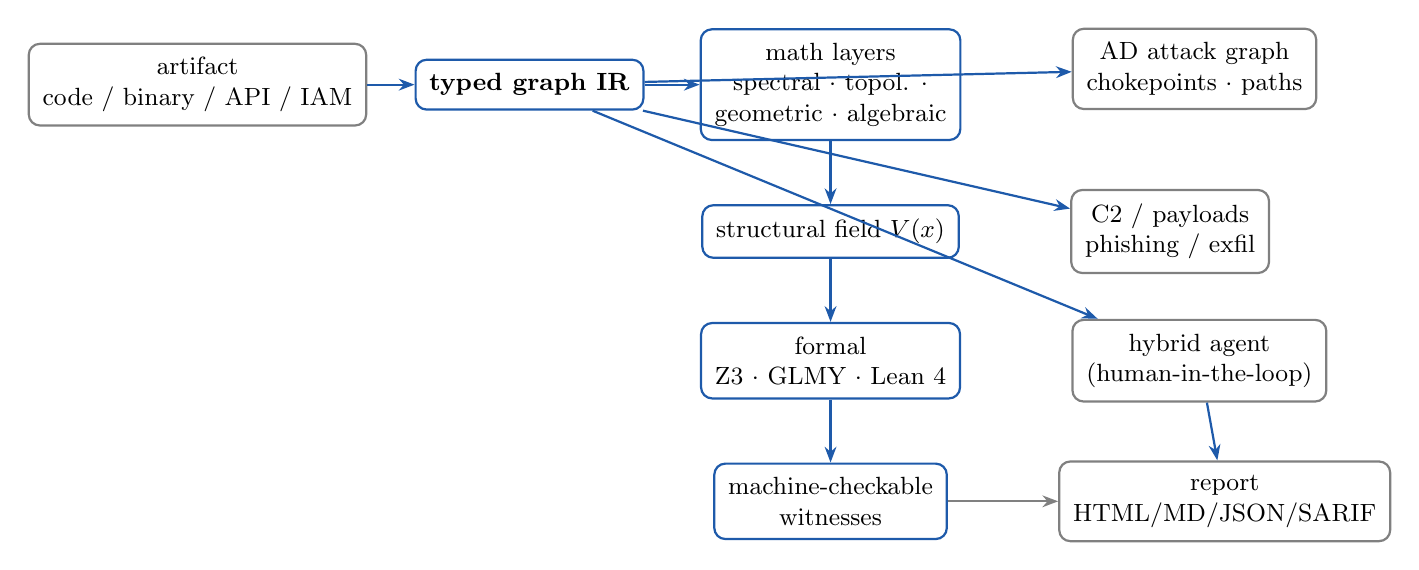
\begin{tikzpicture}[
      box/.style={rectangle, draw=valen, thick, rounded corners, align=center,
                  font=\small, inner sep=5pt},
      soft/.style={rectangle, draw=gray, thick, rounded corners, align=center,
                   font=\small, inner sep=5pt},
      arr/.style={-{Stealth[length=2mm]}, thick, valen},
      ]
    % left: defensive / verifier
    \node[soft] (art) {artifact\\code / binary / API / IAM};
    \node[box, right=6mm of art] (ir) {\textbf{typed graph IR}};
    \node[box, right=7mm of ir] (layers) {math layers\\spectral $\cdot$ topol. $\cdot$\\geometric $\cdot$ algebraic};
    \node[box, below=8mm of layers] (field) {structural field $V(x)$};
    \node[box, below=8mm of field] (verify) {formal\\Z3 $\cdot$ GLMY $\cdot$ Lean 4};
    \node[box, below=8mm of verify] (wit) {machine-checkable\\witnesses};

    % right: offensive / platform
    \node[soft, right=14mm of layers, yshift=2mm] (ad) {AD attack graph\\chokepoints $\cdot$ paths};
    \node[soft, right=14mm of field] (c2) {C2 / payloads\\phishing / exfil};
    \node[soft, right=14mm of verify] (agent) {hybrid agent\\(human-in-the-loop)};
    \node[soft, right=14mm of wit] (report) {report\\HTML/MD/JSON/SARIF};

    \draw[arr] (art) -- (ir);
    \draw[arr] (ir) -- (layers);
    \draw[arr] (layers) -- (field);
    \draw[arr] (field) -- (verify);
    \draw[arr] (verify) -- (wit);
    \draw[arr] (ir) -- (ad);
    \draw[arr] (ir) -- (c2);
    \draw[arr] (ir) -- (agent);
    \draw[arr] (agent) -- (report);
    \draw[arr, gray] (wit) -- (report);
  \end{tikzpicture}
  \caption{One typed IR feeds both a \emph{verifier} (left) and a \emph{red-team
  platform} (right). Findings become witnesses, attack plans, and reports.}
\end{figure}


Everything is built over one deterministic, JSON-serializable typed graph
intermediate representation (IR). Six ingest adapters (Python, Java with
interprocedural/context-sensitive taint, C/C++/Rust/C\#/Go/PHP/Ruby/JavaScript
via a generic C-like engine, binary via \texttt{objdump}/\texttt{angr}, OpenAPI,
IAM, LLM-agent, Solidity) emit the same graph, shared verbatim between the
Python layer and an optional Rust numeric core (with a pure-Python fallback).
Five signal families are fused over it --- algebraic (taint lattice, privilege
levels), spectral (Fiedler), topological (persistent and GLMY directed homology),
geometric (Forman--/Ollivier--Ricci), and formal (Z3, Lean~4) --- and every result
carries a machine-checkable witness under the modeled semantics.

\section{Structural verification}
\label{sec:verification}

\subsection{The boundary on geometric priors}
\label{sec:boundary}
On OWASP Benchmark~1.2 (2740 cases with known ground truth) we ask whether each
signal ranks the vulnerable sink above the safe candidates. A prioritization
oracle computes MRR, R@1, NDCG@$k$, cost curves, a paired permutation test, and
bootstrap confidence intervals. The result is falsifiable and reproducible:
raw taint dominates (MRR $0.894$, AUC $0.895$), the fused structural field is
slightly \emph{worse} ($0.872$, $p=5\times10^{-5}$, 95\% CI $[+0.0157,+0.0294]$),
and spectral ($0.496$) and topological ($0.500$) are at chance while curvature is
below chance ($0.376$). A flat, near-acyclic servlet has no curvature or
persistent topology to exploit, and taint is already near-optimal there.

% Figure: the boundary result (per-signal AUC, chance line)
\begin{figure}[t]
  \centering
  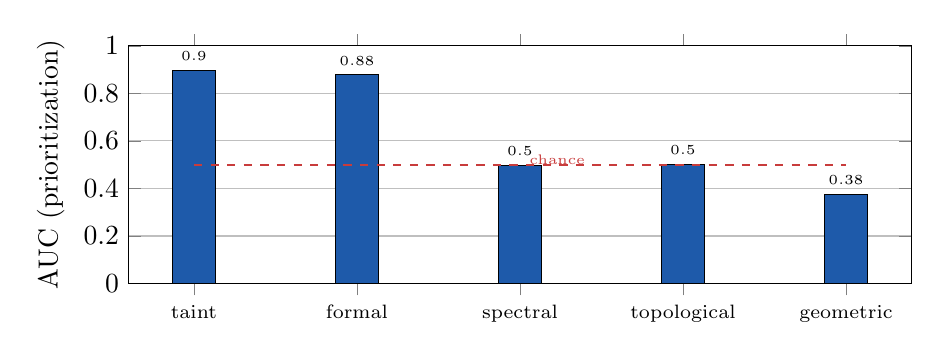
\begin{tikzpicture}
    \begin{axis}[
        ybar, bar width=0.55cm, width=0.95\linewidth, height=4.6cm,
        symbolic x coords={taint, formal, spectral, topological, geometric},
        xtick=data, x tick label style={font=\scriptsize},
        ymin=0, ymax=1.0, ylabel={AUC (prioritization)},
        nodes near coords, every node near coord/.append style={font=\tiny},
        ymajorgrids=true,
      ]
      \addplot[fill=valen] coordinates {
        (taint,0.895) (formal,0.878) (spectral,0.496)
        (topological,0.500) (geometric,0.376)};
      \draw[dashed, valenred, thick] (axis cs:taint,0.5) -- (axis cs:geometric,0.5);
      \node[anchor=west, font=\tiny, valenred] at (axis cs:spectral,0.52) {chance};
    \end{axis}
  \end{tikzpicture}
  \caption{The boundary result: spectral and topological signals are at chance,
  curvature below it; taint is the dominant signal for injection prioritization.}
\end{figure}


\subsection{Authorization, mechanized and operational}
\label{sec:authz}
Let $F:V\to\N$ assign a privilege level; an edge $e=(u,v)$ is an \emph{auth edge}
iff $F(u)<F(v)$. A path with no auth edge satisfies $F(k)\le F(s)$ --- no
privilege escalation --- mechanized in Lean~4. The structural missing-
authorization/BOLA detector flags a function with an HTTP source and a resource
sink but no auth gate: on a curated 39-case corpus it reaches recall $1.0$ /
precision $0.72$ / F1 $0.837$ where taint scores $0$, and a baseline ladder shows
each requirement earns its keep ($0.46\to0.72$). The Z3 verifier checks
$\mathrm{SAT}(\mathrm{owner}(id)\neq session)$ --- an ownership witness that makes
precise that \texttt{login\_required} does not block BOLA, only an
\texttt{owner} predicate does. On crAPI (44 operations, 9 documented BOLA/BFLA
endpoints) an object-reference signal recovers all 9 (recall $1.0$, precision
$0.90$) while the missing-auth check scores $0$, because every BOLA endpoint
\emph{is} authenticated.

% Figure: BOLA/IDOR detector ablation ladder
\begin{figure}[t]
  \centering
  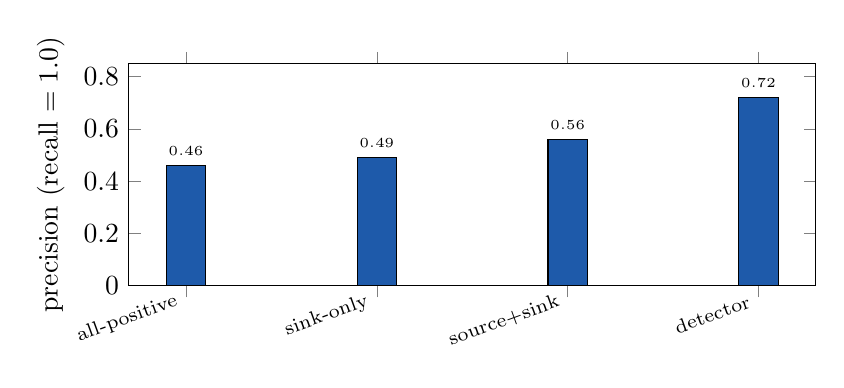
\begin{tikzpicture}
    \begin{axis}[
        ybar, bar width=0.5cm, width=0.85\linewidth, height=4.4cm,
        symbolic x coords={all-positive, sink-only, source+sink, detector},
        xtick=data, x tick label style={rotate=20, anchor=east, font=\scriptsize},
        ymin=0, ymax=0.85, ylabel={precision (recall $=1.0$)},
        nodes near coords, every node near coord/.append style={font=\tiny},
      ]
      \addplot[fill=valen] coordinates {
        (all-positive,0.46) (sink-only,0.49) (source+sink,0.56) (detector,0.72)};
    \end{axis}
  \end{tikzpicture}
  \caption{Each structural requirement of the BOLA/IDOR detector raises precision
  at constant recall: the detector reaches $0.72$ where taint scores $0$.}
\end{figure}


\subsection{Directed path homology}
\label{sec:glmy}
Symmetrizing a directed graph is lossy in both directions: a 2-cycle
$A\to B\to A$ collapses (a missed reentrancy) and a filled triangle becomes a
false cycle. GLMY directed path homology resolves both: recall $1.0$ / precision
$0.75$ on a 12-graph corpus versus $0.5$/$0.5$ symmetrized, and on SmartBugs-
curated smart contracts $0.968$ vs.\ $0.065$ recall. It returns the concrete
$\beta_1$ generator (the cycle's edges) as evidence; its two false positives are
diamond path-space holes, not feedback loops --- $H_1$ is a high-recall,
necessary-but-not-sufficient superset of destructive cycles.

% Figure: directed (GLMY) vs symmetrized homology
\begin{figure}[t]
  \centering
  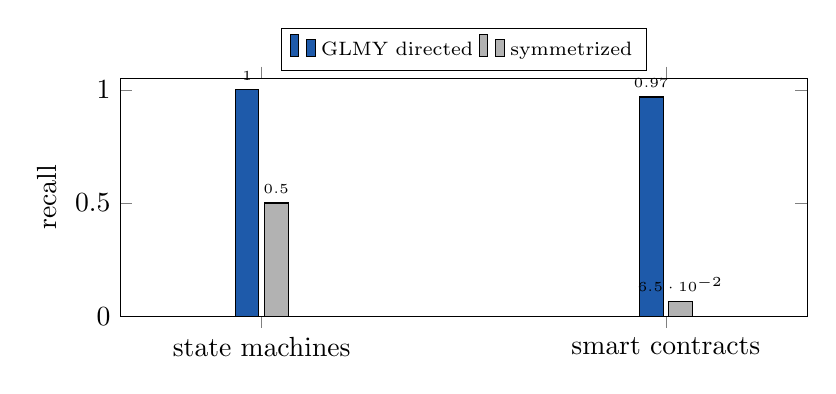
\begin{tikzpicture}
    \begin{axis}[
        ybar, bar width=0.30cm, width=0.85\linewidth, height=4.6cm,
        symbolic x coords={state machines, smart contracts},
        xtick=data, ymin=0, ymax=1.05, ylabel={recall},
        legend style={at={(0.5,1.03)}, anchor=south, legend columns=-1, font=\scriptsize},
        nodes near coords, every node near coord/.append style={font=\tiny},
        enlarge x limits=0.35,
      ]
      \addplot[fill=valen] coordinates {(state machines,1.00) (smart contracts,0.968)};
      \addplot[fill=gray!60]  coordinates {(state machines,0.50) (smart contracts,0.065)};
      \legend{GLMY directed, symmetrized}
    \end{axis}
  \end{tikzpicture}
  \caption{Directed (GLMY) path homology vs.\ symmetrized homology: symmetrization
  collapses the directed 2-cycle, dropping recall from $1.0\to0.5$ on state
  machines and $0.97\to0.065$ on smart contracts.}
\end{figure}


\subsection{The neuro-symbolic arbitration boundary}
\label{sec:neuro}
On a 38-file corpus (29 confirmed findings) the offline heuristic and the
LiteLLM-backed agent agree on detection and ranking on $37/38$ files (agreement
$0.974$), while the LLM changes the CWE on $28\%$ of findings and produces more
concise titles. A spec-mining probe mines a plausible precondition every time
(hallucination $0$) at $0.5$ token recall. The contribution is an architecture ---
LLM proposes, Z3 disposes --- plus its measurement.

\section{Multi-language SAST}
\label{sec:langs}
One generic taint engine (\texttt{clike.py}) drives nine tree-sitter grammars
(C, C++, Rust, C\#, Go, PHP, Ruby, JavaScript/TypeScript), with per-language
\emph{profiles} that declare sources, sinks, sanitizers, and auth gates. The
engine resolves callees (including receivers and scoped names), propagates taint
through straight-line assignments, treats output-parameter sources
(\texttt{fgets}, \texttt{gets}) and pointer declarators, and emits the canonical
IR. A registry (\texttt{categories.py}) unifies severity, CWE, OWASP Top-10,
default CVSS 3.1/4.0 vectors, MITRE tactic and remediation per category, so a
finding is immediately enriched for reporting.

% Figure: one generic engine, nine grammars
\begin{figure}[t]
  \centering
  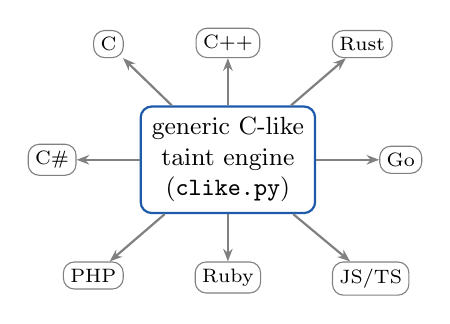
\begin{tikzpicture}[
      box/.style={rectangle, draw=valen, thick, rounded corners, align=center,
                  font=\small, inner sep=4pt},
      lang/.style={rectangle, draw=gray, rounded corners, align=center, font=\scriptsize, inner sep=2.5pt},
      arr/.style={-{Stealth[length=1.6mm]}, gray, thick},
    ]
    \node[box] (engine) {generic C-like\\taint engine\\(\texttt{clike.py})};
    \node[lang, above left=6mm and 2mm of engine] (c) {C};
    \node[lang, above=6mm of engine] (cpp) {C++};
    \node[lang, above right=6mm and 2mm of engine] (rust) {Rust};
    \node[lang, left=8mm of engine] (cs) {C\#};
    \node[lang, right=8mm of engine] (go) {Go};
    \node[lang, below left=6mm and 2mm of engine] (php) {PHP};
    \node[lang, below=6mm of engine] (ruby) {Ruby};
    \node[lang, below right=6mm and 2mm of engine] (js) {JS/TS};
    \draw[arr] (engine) -- (c);  \draw[arr] (engine) -- (cpp);
    \draw[arr] (engine) -- (rust); \draw[arr] (engine) -- (cs);
    \draw[arr] (engine) -- (go);  \draw[arr] (engine) -- (php);
    \draw[arr] (engine) -- (ruby); \draw[arr] (engine) -- (js);
  \end{tikzpicture}
  \caption{One generic taint engine drives nine tree-sitter grammars via
  per-language source/sink/sanitizer profiles; Python, Java (interprocedural) and
  Solidity have dedicated adapters.}
\end{figure}


\section{The red-team platform}
\label{sec:platform}
% Figure: the red-team kill chain
\begin{figure}[t]
  \centering
  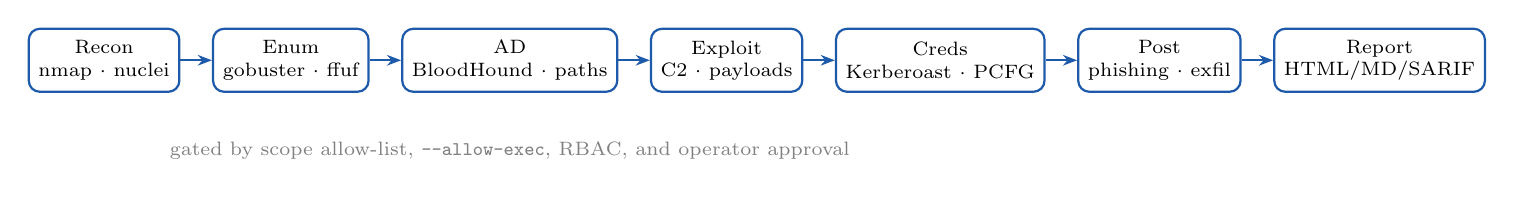
\begin{tikzpicture}[
      box/.style={rectangle, draw=valen, thick, rounded corners, align=center,
                  font=\scriptsize, inner sep=3.5pt, minimum height=8mm},
      arr/.style={-{Stealth[length=1.8mm]}, thick, valen},
    ]
    \node[box] (recon) {Recon\\nmap $\cdot$ nuclei};
    \node[box, right=4mm of recon] (enum) {Enum\\gobuster $\cdot$ ffuf};
    \node[box, right=4mm of enum] (ad) {AD\\BloodHound $\cdot$ paths};
    \node[box, right=4mm of ad] (exploit) {Exploit\\C2 $\cdot$ payloads};
    \node[box, right=4mm of exploit] (creds) {Creds\\Kerberoast $\cdot$ PCFG};
    \node[box, right=4mm of creds] (post) {Post\\phishing $\cdot$ exfil};
    \node[box, right=4mm of post] (report) {Report\\HTML/MD/SARIF};
    \draw[arr] (recon) -- (enum);
    \draw[arr] (enum) -- (ad);
    \draw[arr] (ad) -- (exploit);
    \draw[arr] (exploit) -- (creds);
    \draw[arr] (creds) -- (post);
    \draw[arr] (post) -- (report);
    \node[align=center, font=\scriptsize, below=5mm of ad, gray]
      {gated by scope allow-list, \texttt{--allow-exec}, RBAC, and operator approval};
  \end{tikzpicture}
  \caption{The red-team platform spans the kill chain end-to-end, coordinated by
  the team server and gated by an authorization-first model.}
\end{figure}


\valen\ is a single installable Python package whose server is a multi-user
\emph{team server}: users with roles (\texttt{viewer}/\texttt{operator}/
\texttt{admin}), PBKDF2 sessions, per-route RBAC, engagements with membership,
evidence artifacts, and Server-Sent Events for live operator collaboration, all
persisted in SQLite. The red-team surface spans the kill chain:

\begin{itemize}[itemsep=1pt]
\item \textbf{Recon / enumeration} --- nmap, masscan, gobuster, ffuf, nuclei
  wrappers with stealth profiles and CVE/KEV/EPSS intelligence.
\item \textbf{Active Directory} --- BloodHound/SharpHound ingestion into the IR,
  tier-0 attack paths, Kerberoast/AS-REP selection, GPP \texttt{cpassword}
  decryption, and impacket/kerbrute/hashcat command builders.
\item \textbf{C2 and payloads} --- Sliver integration (gRPC-first, shell
  fallback), msfvenom/handler/HTA planners, GoPhish and exfiltration planners.
\item \textbf{Hybrid agent} --- a deterministic kill-chain planner with an
  operator approval queue; intrusive actions require explicit \texttt{--authorize}.
\item \textbf{Reporting} --- HTML / Markdown / JSON / SARIF with CVSS 3.1/4.0 and
  CVE/KEV/EPSS enrichment.
\end{itemize}

Everything offensive is gated by a scope allow-list (loopback by default), an
execution allow-list (\texttt{--allow-exec}), and per-operator roles --- an
\emph{authorization-first} model, not an afterthought.

\section{Attack-graph mathematics}
\label{sec:math}
The IR is a typed directed multigraph $G=(V,E)$ over principals. Four families of
methods are layered over it.

\subsection{Flow: chokepoints and disjoint plans}
\textbf{Menger min-cut.} Given entry set $S$ and target set $T$, we compute the
minimum vertex set whose removal separates them, by $s$-$t$ max flow on the
vertex-split graph (each $v$ becomes $v_{\mathrm{in}}\to v_{\mathrm{out}}$ of
capacity $1$; sources/targets unbounded) with Edmonds--Karp. The saturated split
edges on the source side of the residual graph are the \emph{obligatory
chokepoints}. A flow $\geq\infty$ means a source is directly adjacent to a target
(min-cut $0$).

\textbf{Min-cost flow.} With a per-edge cost model (stealth + effort;
$\text{MemberOf}=1$, $\text{DCSync}=5$), we send $k$ units at minimum cost via
successive shortest augmenting paths. Internal vertices have capacity $1$, so the
result is a set of \emph{vertex-disjoint} cheapest routes --- ``with $k$
compromises, the $k$ cheapest independent ways in''.

\textbf{Articulation points and bridges} (Tarjan, on the symmetrized graph) rank
the most disruptive principals and links --- the attacker/disruption view ---
while the directed min-cut is the defender/hardening view.

% Figure: Active Directory attack graph with chokepoint and least-cost path
\begin{figure}[t]
  \centering
  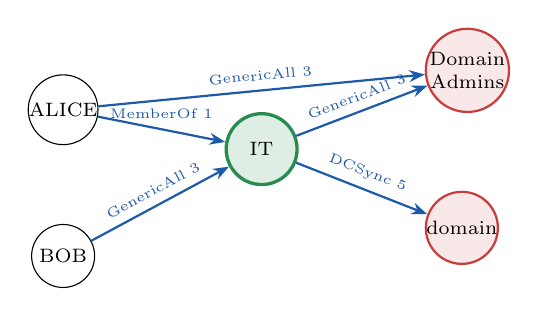
\begin{tikzpicture}[
      n/.style={circle, draw, inner sep=0pt, minimum size=8mm, font=\scriptsize, align=center},
      target/.style={circle, draw=valenred, thick, fill=valenred!12, inner sep=0pt, minimum size=9mm, font=\scriptsize, align=center},
      chok/.style={circle, draw=valengreen, very thick, fill=valengreen!15, inner sep=0pt, minimum size=9mm, font=\scriptsize, align=center},
      arr/.style={-{Stealth[length=2mm]}, thick, valen, font=\tiny},
    ]
    \node[n] (alice) {ALICE};
    \node[n, below=10mm of alice] (bob) {BOB};
    \node[chok, right=16mm of alice, yshift=-5mm] (it) {IT};
    \node[target, right=16mm of it, yshift=10mm] (da) {Domain\\Admins};
    \node[target, right=16mm of it, yshift=-10mm] (dom) {domain};

    \draw[arr] (alice) -- node[above, sloped]{GenericAll $3$} (da);
    \draw[arr] (alice) -- node[above]{MemberOf $1$} (it);
    \draw[arr] (bob) -- node[above, sloped]{GenericAll $3$} (it);
    \draw[arr] (it) -- node[above, sloped]{GenericAll $3$} (da);
    \draw[arr] (it) -- node[above, sloped]{DCSync $5$} (dom);
  \end{tikzpicture}
  \caption{The AD attack graph: with entry \texttt{BOB}, \texttt{IT} is the
  Menger min-cut chokepoint (min-cut $1$); \texttt{ALICE} reaches Domain Admins
  directly (min-cut $0$). Least-cost plans: \texttt{ALICE}$\to$Domain Admins
  ($3.0$) and \texttt{ALICE}$\to$\texttt{IT}$\to$domain ($6.0$); \texttt{BOB} is
  certified unreachable to Domain Admins.}
  \label{fig:attackgraph}
\end{figure}


\subsection{Probability: hitting time}
Model the graph as an absorbing Markov chain: targets are absorbing and each
transient node transitions uniformly over out-neighbours. The hitting probability
satisfies
\[
h(u) \;=\; \mathbb{1}[u\in T] \;+\; \mathbb{1}[u\notin T]\cdot
\frac{1}{\deg^+(u)}\sum_{v:\,u\to v} h(v),
\]
computed by value iteration or \emph{exactly} by Gaussian elimination on
$(I-Q)h=r$. In the toy corpus an entry with three out-edges and one route to the
target scores $\tfrac13$, a direct entry $1$ --- a probabilistic risk ranking
distinct from boolean reachability.

\subsection{Formal synthesis: minimal-cost exploit plans}
Boolean reachability answers \emph{is it reachable?}; we answer \emph{what is the
cheapest ordered sequence of actions?} Model the graph as a transition system
\[
\mathrm{has}(s{+}1,n)\;\equiv\;\mathrm{has}(s,n)\;\vee\;
\bigvee_{e:\,m\to n}\bigl(\mathrm{taken}_e\wedge\mathrm{has}(s,m)\bigr),
\]
with entries compromised at step $0$, and ask \texttt{z3.Optimize} to minimize
$\sum_e \mathrm{taken}_e\cdot \mathrm{cost}(e)$ subject to reaching the target
within $k$ steps. Reconstructing the ordered sequence yields the
technique-by-technique narrative. We extend it to \textbf{AND-preconditions}:
compound actions $\{\mathrm{sources}\to\mathrm{target}\}$ that fire only when all
sources are compromised (e.g.\ DCSync needs Domain Admins \emph{and} a session on
a Domain Controller).

\subsection{Password guessing: PCFG}
We implement Weir's probabilistic context-free grammar: tokenize passwords into
$L/D/S$ runs; the base structure (e.g.\ $L_6D_4S_1$) is the non-terminal, and
terminals are keyed by $(\text{class},\text{length})$ so no cross-length mixing.
$P(\mathrm{guess})=P(\mathrm{structure})\cdot\prod P(\mathrm{terminal})$, and
guesses are emitted in strictly decreasing probability by a best-first walk. The
training corpus is a cracked hashcat potfile.

\section{Evaluation}
\label{sec:eval}

\subsection{Autonomous pentest against OWASP crAPI}
Against a fresh crAPI 1.1.5 lab the autonomous agent solves \textbf{18/18}
documented challenges --- BOLA/BFLA, mass assignment, SSRF, NoSQL/SQL injection,
JWT forgery, password reset, rate limit, and three LLM prompt-injection
challenges (routed through a local LiteLLM proxy). The BOLA detector reaches
recall $1.0$ / precision $0.90$ / F1 $0.947$.

\subsection{Active Directory toy corpus}
On a synthetic SharpHound corpus the layers compose (Figure~\ref{fig:attackgraph}):
with entry \texttt{BOB}, min-cut $1$ at the intermediate group \texttt{IT}; with
entry \texttt{ALICE} (direct GenericAll on Domain Admins), min-cut $0$; hitting
$\texttt{ALICE}=1.0$, $\texttt{BOB}=\tfrac13$; synthesis yields
\texttt{ALICE}$\xrightarrow{\text{GenericAll/T1098}}$ Domain Admins (cost $3.0$)
and \texttt{ALICE}$\xrightarrow{\text{MemberOf}}\,$\texttt{IT}
$\xrightarrow{\text{DCSync/T1003.006}}$ domain (cost $6.0$), while \texttt{BOB} is
certified \emph{unreachable} to Domain Admins.

\subsection{Results at a glance}
\begin{center}\small
\begin{tabular}{@{}lll@{}}
\toprule
\textbf{Contribution} & \textbf{Metric} & \textbf{Result} \\
\midrule
C1 boundary & taint vs.\ fused field (MRR) & $0.894$ vs.\ $0.872$ ($p=5\times10^{-5}$) \\
C2 authorization & crAPI BOLA/IDOR (recall / precision) & $1.0$ / $0.90$ \\
C2 authorization & curated BOLA ladder (precision) & $0.46\to0.72$ \\
C3 directed homology & GLMY vs.\ symmetrized (contracts) & $0.968$ vs.\ $0.065$ recall \\
C4 arbitration & detection/ranking agreement & $0.974$; CWE $28\%$ \\
C5 languages & SAST adapters & $9$ languages, $1$ engine \\
C6 platform & team server & roles, RBAC, SSE, SQLite \\
C7 math & chokepoints / min-cost flow / hitting / synthesis / PCFG & implemented \\
Red team & autonomous crAPI challenges & $18/18$ solved \\
\bottomrule
\end{tabular}
\end{center}

% Figure: autonomous pentest score (18/18)
\begin{figure}[t]
  \centering
  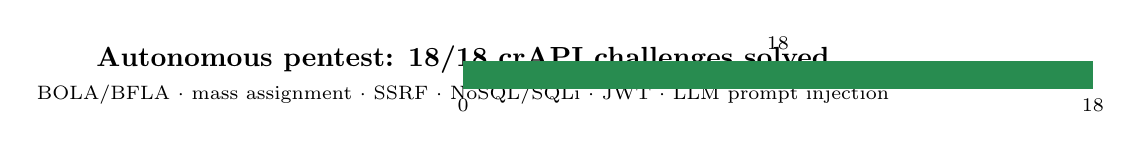
\begin{tikzpicture}
    \node[font=\normalsize, align=center] {\textbf{Autonomous pentest: 18/18 crAPI challenges solved}\\
      {\scriptsize BOLA/BFLA $\cdot$ mass assignment $\cdot$ SSRF $\cdot$ NoSQL/SQLi $\cdot$ JWT $\cdot$ LLM prompt injection}};
    \draw[gray!30, line width=10pt] (0,0) -- (8,0);
    \draw[valengreen, line width=10pt] (0,0) -- (8,0);
    \node[below] at (0,-0.18) {\scriptsize 0};
    \node[below] at (8,-0.18) {\scriptsize 18};
    \node[above, font=\scriptsize] at (4,0.2) {18};
  \end{tikzpicture}
  \caption{The autonomous agent solves all 18 documented crAPI challenges,
  including three LLM prompt-injection challenges routed through a local LiteLLM
  proxy.}
\end{figure}


\section{Limitations and ethics}
The evaluations are a single real API plus curated corpora, not public
benchmarks; the structural detector over-approximates; the Z3 witness holds under
the \emph{modeled} semantics; the pure-Python numeric fallback is an honest
approximation of the Rust core; the PCFG prior is only as good as its corpus. The
platform is an \emph{authorized-engagement} tool: scope is loopback by default,
execution is behind \texttt{--allow-exec}, intrusive actions require operator
approval, and every module carries a ``for authorized engagements only'' notice.

\section{Conclusion}
\valen\ joins a measured defensive thesis --- structural invariants verify
authorization, state, and trust properties, not injection prioritization --- with
an offensive platform whose differentiator is \emph{quantitative attack-graph
mathematics}: chokepoints, least-cost and disjoint plans, exact hitting
probabilities, minimal-cost exploit synthesis with AND-preconditions, and a PCFG
password prior. All code is installable, tested ($383$ tests), and documented, and
all results are reproducible from the included artifacts.

\bibliographystyle{plain}
\nocite{*}
\end{document}
